%%% ---------------------------------------------------------------------------------
%%% Vorlage Abschlussarbeit (LaTeX)
%%% 
%%% V1   03/2017, Stefan Etschberger (HSA)
%%% V1.1 04/2021, rnw-hack für biblatex-run
%%% V2   05/2021, Titelblatt und Erweiterungen: Stefan Jansen (HSA)
%%% V2.1 05/2021, Trennung von R-Support und einfachem LaTeX: Phillip Heidegger (HSA)
%%% V2.2 01/2024, Anpassung an THA-Layout
%%% V3   01/2024, I18n
%%% V3.1 10/2024, Phillip Heideger, Online Version präferiert, Reparatur langes Inhaltsverzeichnis,
%%%               Erklärung Referenzen, blau für Refs & Links
%%% ---------------------------------------------------------------------------------
\documentclass[12pt,a4paper%
              ,oneside     % fuer PDF-Abgabe, bei Druck twoside
              ,titlepage
              ,DIV=13
              ,headinclude
              ,footinclude=false%
              ,cleardoublepage=empty%
              ,parskip=half,
              BCOR=0mm,
              ]{scrreprt}

\usepackage[utf8]{inputenc}
\usepackage[T1]{fontenc}

\usepackage[authorName={}
           ,authorEnrolmentNo={}
           ,authorStreet={}
           ,authorZip={}
           ,authorCity={}
           ,authorEMail={}
           ,authorPhone= {}
           ,authorSignaturePlace={}
           ,studyProgram={Mathematik}
           ,thesisType={Dokumentation}
           ,thesisTitle={NoSQL: Umsetzung der Semesteraufgabe mit Google Firestore}
           ,studyDegree=%
%                        {{Bachelor of Arts}}
%                        {{Bachelor of Engeneering}}
                        {{Bachelor of Science (B.\,Sc.)}}
%                        {{Master of Arts}}
%                        {{Master of Engeneering}}
%                        {{Master of Science (M.\,Sc.)}}
           ,faculty=% 
%                     {{Fakultät für \\ Angewandte \\ Geistes-  und  \\ Naturwissenschaften}}
%                     {{Fakultät für \\ Architektur und \\ Bauwesen}}
%                     {{Fakultät für \\ Elektrotechnik}}
%                     {{Fakultät für \\ Gestaltung}}
                      {{Fakultät für \\ Informatik}}
%                     {{Fakultät für \\ Maschinenbau und \\ Verfahrenstechnik}}, showDiesel=true
%                     {{Fakultät für \\ Wirtschaft}}
%           ,topicAssignment={\today}
%           ,submissionDate={\today}
%           ,defenseDate={\today}
%           ,nonDisclosure={false}
           ,supervisor={Prof.~Dr.~Frank N. Stein}
%           ,supervisorDeputy={Prof.~Dr.~Mario Huana}
%           ,language={en}
           ]{THA-docu}

% ====== mögliches Setup fürs PDFs =======
\hypersetup{
  colorlinks=true,
  allcolors = THAi-Blue, % oder THAred ??
  linktocpage  
}
% Siehe:
% https://ctan.net/macros/latex/contrib/hyperref/doc/hyperref-doc.pdf
% S. Kap. 5, S. 10 ff

% Ohne diese Zeile: Mit klickbaren links
% \hypersetup{draft}


% Literaturdatenbank (.bib-Datei) aus Citavi o.ä.
\bibliography{Literatur_docu}

\graphicspath{{Bilder/}}

\usepackage[font=small,labelfont=bf]{caption}
\DeclareCaptionLabelFormat{something}{#2.#1.}
\captionsetup[lstlisting]{labelformat=something}

\usepackage{chngcntr}
\usepackage{float}

\counterwithout{figure}{chapter}
\Urlmuskip=0mu plus 1mu  % erlaubt Umbrüche an beliebigen Stellen

\begin{document}

% Sprachauswahl zum Umschalten innerhalb des Textes. 
% Alternativen: \thesisLanguage, ngerman, english
\selectlanguage{\thesisLanguage}

\pagenumbering{roman}
\setcounter{page}{1}

\THAtitlepage

\tableofcontents

%%% --------------------------------------------------
%%% Ab hier: Inhalt
%%% --------------------------------------------------

\setcounter{page}{1}
\pagenumbering{arabic}

\chapter{Ausgangssituation}
\label{einleitung}

In unserer neuen Position im Datenbank-Team haben wir von unserem Vorgänger eine relationale Kurs-Datenbank übernommen. Laut Vorgabe des Managements soll diese nun in eine moderne NoSQL-Datenbank überführt werden.

Da keine strukturierte Übergabe stattfand, stand uns lediglich ein SQL-Dump der alten Datenbank zur Verfügung. Um die Datenstruktur besser zu verstehen und einen Überblick über die enthaltenen Tabellen und deren Beziehungen zu gewinnen, haben wir diesen Dump zunächst in ein Entity-Relationship-Diagramm (ERD) überführt.

Abbildung~\ref{fig:enr-old} zeigt das daraus entstandene ER-Diagramm, das insgesamt neun relationale Tabellen umfasst:

\begin{figure}[htbp]
	\centering
	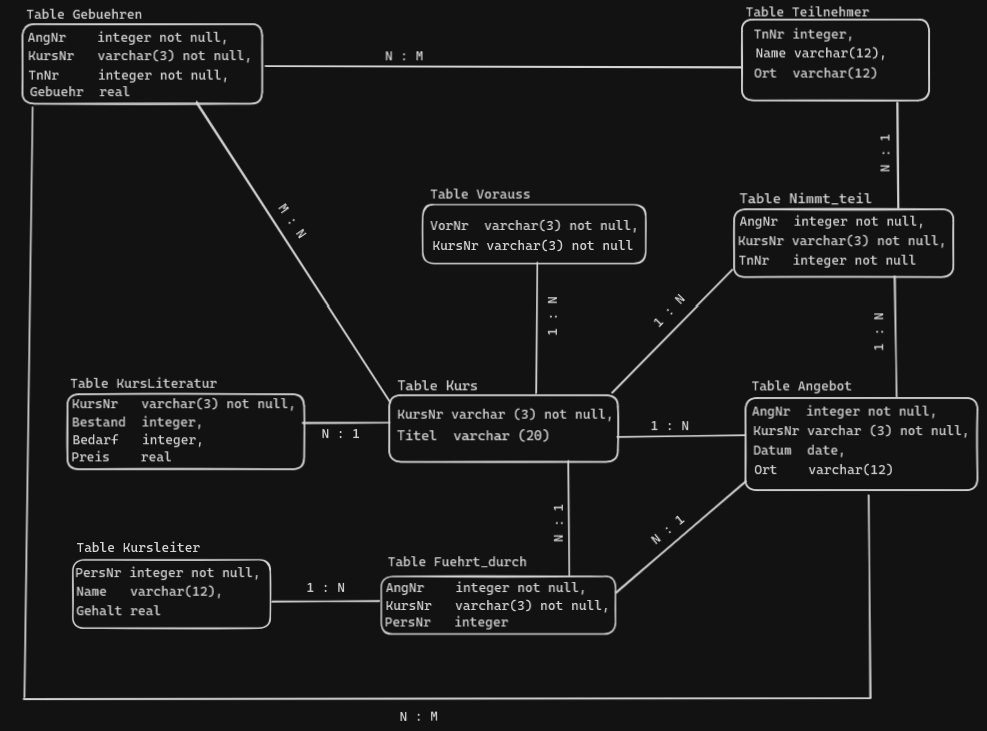
\includegraphics[width=\dimexpr0.8\linewidth]{img/SQL_DUMP_ERM.png}
	\caption{Entity-Relationship-Diagramm der ursprünglichen relationalen Struktur}
	\label{fig:enr-old}
\end{figure}

Auf Basis dieser Analyse mussten wir uns für eine NoSQL-Datenbank entschieden. Die Entscheidung und die Gründe für die jeweilige NoSQL-Datenbank wird nachfolgend beschrieben in Kapitel~\ref{entscheidung-chapter} (\glqq Entscheidung für eine NoSQL-Datenbank\grqq{}).

\chapter{Entscheidung für eine NoSQL-Datenbank}
\label{entscheidung-chapter}

Zur Auswahl einer geeigneten NoSQL-Datenbank haben wir zunächst das \textit{DB-Engines Ranking} (\url{https://db-engines.com/en/ranking}) als Orientierungshilfe herangezogen. Dieses Ranking bietet eine fundierte Übersicht über die aktuell am weitesten verbreiteten Datenbanktechnologien.

Nach einer kurzen Recherche hinsichtlich Verbreitung, Dokumentation und Community-Support fiel unsere Wahl auf \textbf{Google Cloud Firestore}. Ausschlaggebend war neben den technischen Eigenschaften, Google als Entwickler und der guten Integration in das Node.js-Ökosystem auch unser persönliches Interesse an der Arbeit mit Firebase-Technologien.

\section{Google Cloud Firestore}

Google Cloud Firestore ist eine dokumentenbasierte NoSQL-Datenbank, in der Daten in sogenannten \textit{Collections} organisiert sind. Jede \textit{Collection} kann beliebig viele \textit{Dokumente} enthalten, die wiederum hierarchisch strukturierte \textit{Sub-Collections} besitzen können. 

Die einzelnen Dokumente bestehen aus Feldern in Form von Schlüssel-Wert-Paaren und ähneln in ihrer Struktur stark \textit{JSON-Objekten}. Dieses flexible Datenmodell ermöglicht die effiziente Speicherung von semistrukturierten Informationen.

Zu den zentralen Merkmalen von Firestore gehören die Unterstützung verschachtelter Datenstrukturen, Arrays, Referenzen auf andere Dokumente sowie spezielle Datentypen wie Zeitstempel. Dadurch lassen sich auch komplexe, objektähnliche Datenmodelle direkt und modellnah abbilden \cite{Kesavan.2023, Firebase.2025, FirebaseDatenmodell.2025}. Nachfolgend zeigt Abbildung~\ref{fig:struktur-example} ein Datenstruktur-Beispiel in Firestore:

\begin{figure}[H]
	\centering
	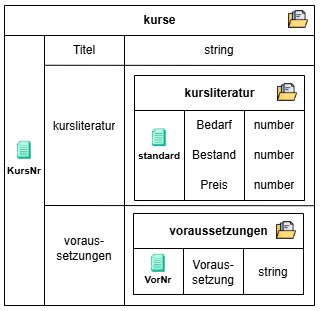
\includegraphics{img/struktur_ausschnitt.png}
	\caption{Beispiel einer dokumentenbasierten Firestore Datenstruktur}
	\label{fig:struktur-example}
\end{figure}

Abbildung~\ref{fig:struktur-example} zeigt hierbei die \textit{Collection} kurse, bei der die \textit{Dokumente} jeweils einen Titel als string beinhalten und zwei \textit{Sub-Collections}, die wiederum ihre eigenen \textit{Dokumente} mit Schlüssel-Wert-Paare beinhalten. Die konkrete vollständige Umsetzung dieser Struktur in unserem Projekt wird in Kapitel~\ref{struktur-chapter} (\glqq Aufbau der Datenstruktur\grqq{}) ausführlich dargestellt.

\section{Abfragesprache von Firestore}
\label{sprache-firestore}

Die Standardabfragesprache von Google Cloud Firestore ist keine deklarative Sprache wie SQL, sondern eine methodenbasierte API, die über verschiedene Programmiersprachen hinweg verfügbar ist. Firestore stellt hierfür offizielle SDKs bereit, unter anderem für JavaScript, TypeScript, Python, Java und Kotlin \cite{GoogleCloudQueries.2025}.

Die Interaktion mit der Datenbank erfolgt über eine Befehlskette aus Methodenaufrufen, mit denen sich Daten lesen, filtern, sortieren und paginieren lassen. Dabei orientieren sich die Methoden am zugrunde liegenden dokumentenbasierten Modell und bieten eine intuitive Möglichkeit, auf Daten zuzugreifen.

Abbildung~\ref{fig:code-example-0} zeigt ein einfaches Beispiel für eine Abfrage in Firestore mit JavaScript. Hier wird nach allen Städten gesucht, bei denen das Feld \textit{capital} auf \textit{true} gesetzt ist, sortiert nach der Bevölkerungszahl:

\begin{figure}[H]
	\centering
	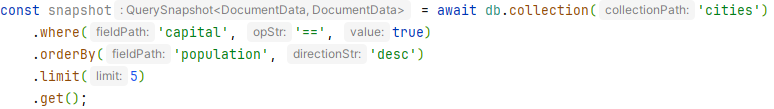
\includegraphics[width=\linewidth]{img/code_example_0.png}
	\caption{Beispiel einer Abfrage in Firestore}
	\label{fig:code-example-0}
\end{figure}

Im Gegensatz zu SQL müssen bei dieser Art von Abfragen Joins, Aggregationen und komplexere Operationen vom Client übernommen werden. Das bedeutet, dass manche Auswertungen – wie etwa das Zusammenführen mehrerer Datensätze – durch zusätzliche Logik im Anwendungscode umgesetzt werden müssen.

In unserem Projekt haben wir uns bewusst für die Verwendung von \textbf{TypeScript} entschieden, um die Stärken der Firestore-API mit statischer Typprüfung zu kombinieren. Dies war insbesondere im Hinblick auf die Datenmigration aus der relationalen Struktur von Vorteil, da wir so die ursprünglichen Datentypen in Form von Interfaces abbilden und validieren konnten.

Wie genau wir mithilfe von TypeScript und sogenannten \textit{Convertern} eine durchgehende Typsicherheit im Zugriff auf Firestore erreicht haben, wird ausführlich in Kapitel~\ref{typ-sicherheit-chapter} (\glqq Typsicherheit und Abfragen mit TypeScript\grqq{}) erläutert.

\section{Lokale Nutzung}

Da Google Cloud Firestore eine cloudbasierte Datenbank ist, standen wir vor der Herausforderung, sie lokal zu betreiben – denn die Nutzung einer Cloud-Lösung war in unserem Fall nicht zulässig. Für diesen Zweck stellt Firebase die sogenannte \textit{Local Emulator Suite} zur Verfügung. Dabei handelt es sich um eine Sammlung von Dienstemulatoren, die das Verhalten der echten Firebase-Dienste lokal nachbilden \cite{EmulatorSuite.2025}.

Für unser Projekt reichte der Einsatz des Firestore-Emulators sowie der zugehörigen Benutzeroberfläche aus. Die Einrichtung erfolgte lokal durch die Installation von \textit{Node.js}, dem \textit{Java JDK} sowie der \textit{Firebase CLI}. Mit wenigen Konfigurationsbefehlen ließ sich anschließend die erforderliche Datei \textit{firebase.json} generieren. Dieses Setup entspricht dem von Firebase empfohlenen Vorgehen für die lokale Entwicklung \cite{EmulatorInsall.2025}.

Abbildung~\ref{fig:emulator-ui} zeigt einen Ausschnitt aus der Benutzeroberfläche des Emulators:

\begin{figure}[H]
	\centering
	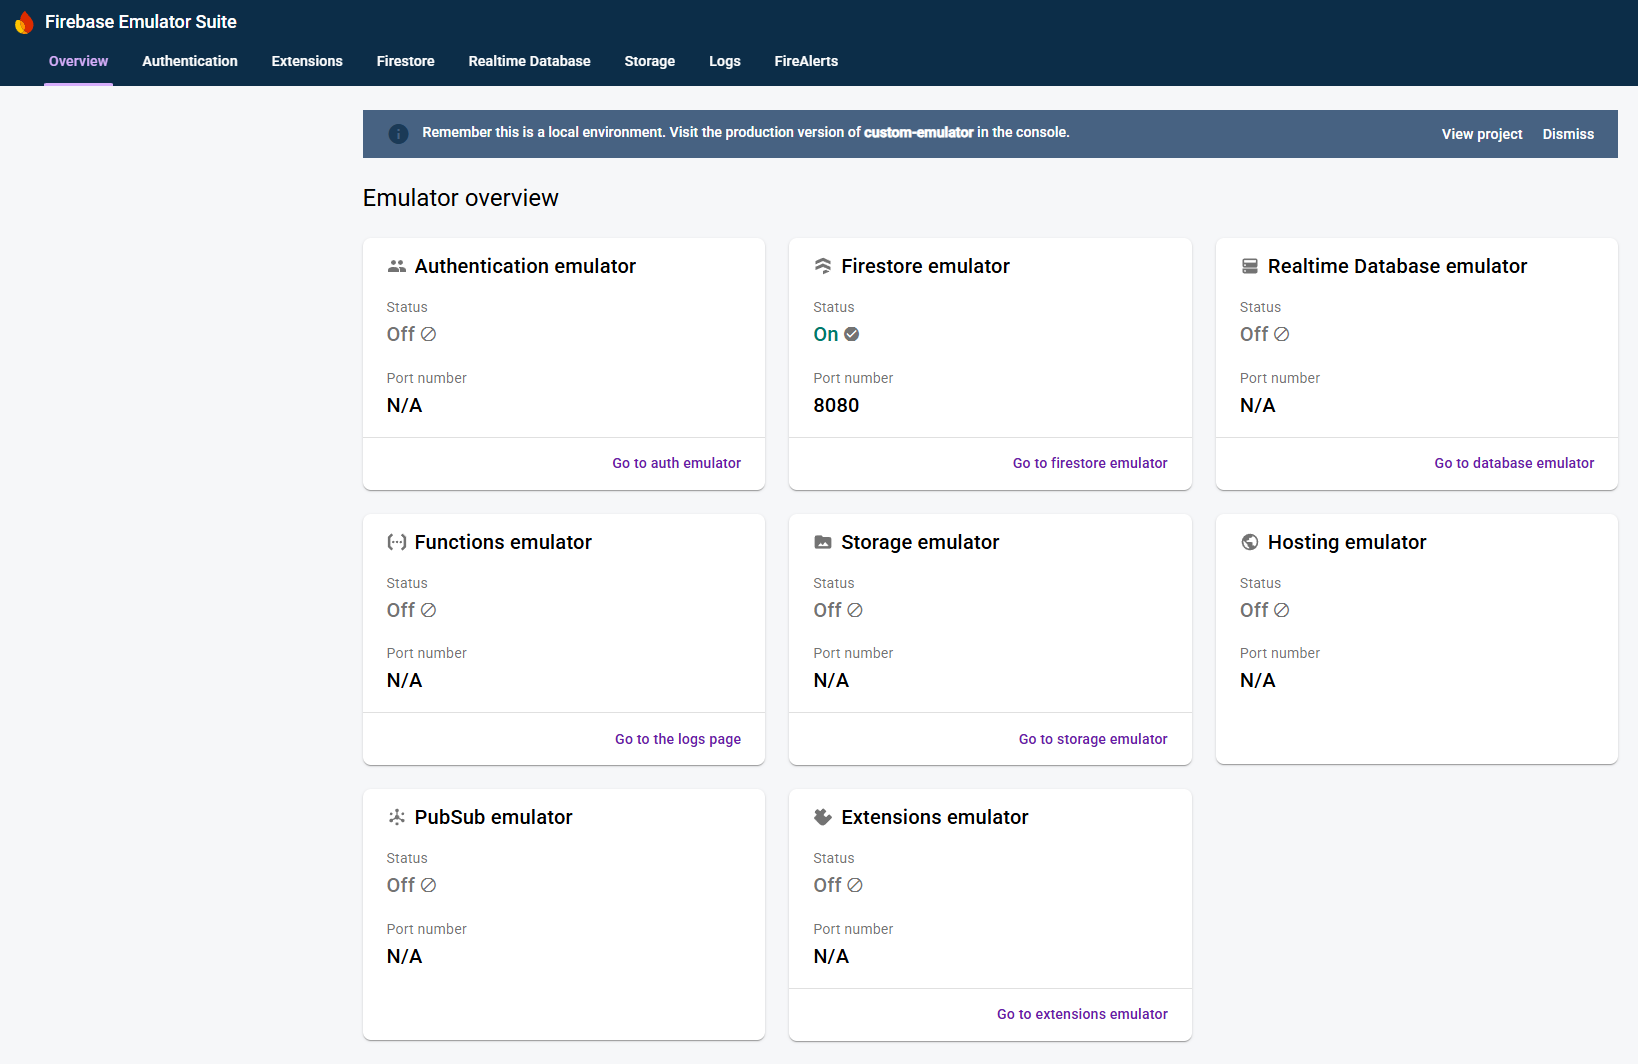
\includegraphics[width=\linewidth]{img/emulator_ui.png}
	\caption{Auszug aus der UI der Local Emulator Suite}
	\label{fig:emulator-ui}
\end{figure}

\subsection{Versuchter alternativer Ansatz zur lokalen Nutzung}

Neben der empfohlenen lokalen Installation der Emulator Suite haben wir auch versucht, die Firestore-Emulatorumgebung mithilfe von Docker bereitzustellen. Ziel war es, die notwendigen Tools nicht direkt auf unseren eigenen Systemen installieren zu müssen.

Dazu haben wir verschiedene Beiträge, Artikel und GitHub-Repositories recherchiert und unterschiedliche Ansätze ausprobiert, unter anderem:

\begin{enumerate}
	\item \url{https://github.com/PathMotion/firestore-emulator-docker}
	\item \url{https://hub.docker.com/r/mtlynch/firestore-emulator/}
	\item \url{https://medium.com/@jens.skott_65388/simplifying-firebase-emulation-with-docker-a-guide-to-local-development-and-testing-0c3c33fd92c7}
	\item \url{https://github.com/ridedott/firestore-emulator-docker}
\end{enumerate}

Diese verschiedenen Ansätze haben unterschiedlichen Projektmitglieder versucht und jeder ist auf andere Probleme gestoßen. Manche hatten bereits Probleme bei der Installation und haben zu keinem Zeitpunkt einen lauffähigen Docker erreicht und manche hatten Probleme bei der Anwendung des Containers. Dabei ließ sich die Emulator Suite zwar innerhalb eines Docker-Containers starten und auch die Benutzeroberfläche aufrufen, jedoch traten in der praktischen Nutzung erhebliche Einschränkungen auf. Das Hauptproblem bestand darin, dass der Zugriff auf die Datenbank aus externen Skripten heraus nicht zuverlässig funktionierte – insbesondere die Weiterleitung der Ports verursachte Schwierigkeiten.

Eine alternative Lösung wäre dazu gewesen, sämtliche Skripte direkt innerhalb des Containers auszuführen. Dieses Vorgehen erschien uns jedoch in Bezug auf Wartbarkeit, Entwicklungsfluss und auf Grund der Tatsache, dass andere Projektmitglieder den Docker nicht ausführen konnten, zu umständlich. Aufgrund dieser Einschränkungen haben wir uns letztlich für den von Firebase vorgesehenen Weg mit lokaler Installation entschieden, der sich als unkompliziert und stabil erwiesen hat.

\chapter{Aufbau der Datenstruktur}
\label{struktur-chapter}

Für die Überführung der in Kapitel~\ref{einleitung} beschriebenen relationalen Struktur haben wir die Vorteile eines dokumentenbasierten Datenmodells – wie es Google Firestore bietet – gezielt genutzt. Die finale Datenstruktur ist dabei nicht von Anfang an in ihrer jetzigen Form entstanden, sondern wurde im Laufe der Projektarbeit mehrfach überarbeitet und optimiert. Ziel war es, eine Lösung zu entwickeln, die sowohl den ursprünglichen Datenbeziehungen gerecht wird als auch eine effiziente Umsetzung der geforderten Abfragen ermöglicht.

Die resultierende Struktur ist in Abbildung~\ref{fig:structure} visualisiert:

\begin{figure}[H]
	\centering
	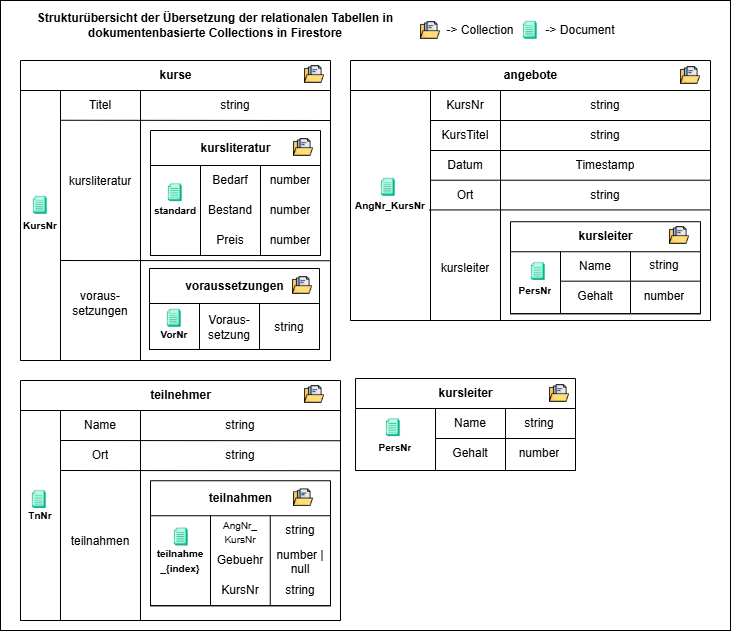
\includegraphics[width=\dimexpr0.9\linewidth]{img/StrukturFirestore.png}
	\caption{Struktur der Daten in Firestore}
	\label{fig:structure}
\end{figure}

Aus den insgesamt neun relationalen Tabellen wurden vier \textit{Haupt-Collections} abgeleitet: \textit{kurse}, \textit{angebote}, \textit{teilnehmer} und \textit{kursleiter}. Dabei wurden einige ursprünglich eigenständige Tabellen als \textit{Sub-Collections} integriert:

\begin{itemize}
	\item In \textit{kurse} befinden sich die \textit{Sub-Collections} \textit{kursliteratur} (ursprünglich: \textit{KursLiteratur}) und \textit{voraussetzungen} (ursprünglich: \textit{Vorauss}).
	\item In \textit{teilnehmer} ist die \textit{Sub-Collection} \textit{teilnahmen} untergebracht (ursprünglich: \textit{Nimmt\_teil}), wobei die ehemals separate Tabelle \textit{Gebuehren} nun als Feld innerhalb eines \textit{teilnahme Dokuments} gespeichert ist.
	\item Die \textit{Collection kursleiter} entspricht nahezu direkt der alten Tabelle gleichen Namens.
	\item Die \textit{Collection angebote} wurde am stärksten angepasst: Neben der \textit{Sub-Collection} \textit{kursleiter}, in der relevante Kursleiterdaten (redundant) gespeichert sind, wird dort zusätzlich der \textit{KursTitel} direkt im Angebot abgelegt.
\end{itemize}

Die redundante Speicherung des Kurstitels sowie der Kursleiterdaten wurde bewusst gewählt. In Firestore sind komplexe \textit{JOINs}, wie sie in relationalen Datenbanken üblich sind, nicht möglich. Um performante Abfragen zu ermöglichen und unnötige Mehrfachabfragen zu vermeiden, ist diese strategische Denormalisierung sogar empfohlen und gilt als \textit{Best Practice} im Umgang mit NoSQL-Datenbanken, um bestimmte, häufig vorkommende Abfragen um bis zu 50\% zu beschleunigen \cite{Estuary.2025, MoldStud.2025}.

Insgesamt entspricht die von uns gewählte Struktur dem Paradigma einer dokumentenorientierten Datenbank. Sie erwies sich im Verlauf der Umsetzung als robust und praxistauglich, insbesondere im Hinblick auf die Bearbeitung der gestellten Aufgaben. Gleichzeitig bringt die Entscheidung für redundante Datenhaltung gewisse Herausforderungen mit sich – insbesondere bei \textit{update}- und \textit{delete}-Operationen. Diese Aspekte werden im Kapitel~\ref{update-delete-chapter} (\glqq Herausforderungen bei den Update- \& Delete-Abfragen\grqq{}) näher erläutert.

\chapter{Typsicherheit und Abfragen mit TypeScript}
\label{typ-sicherheit-chapter}

Wie bereits in Kapitel~\ref{sprache-firestore} erwähnt, haben wir uns bei der Implementierung für \textbf{TypeScript} als Abfragesprache entschieden. Der Hauptgrund dafür war, dass Firestore standardmäßig keine Typsicherheit bietet. Das Datenbanksystem selbst ist schemalos, sodass die Validierung von Datentypen vollständig in der Anwendungsschicht erfolgen muss.

Da wir möglichst nah an den Datentypen der ursprünglichen relationalen Struktur bleiben wollten, haben wir in TypeScript entsprechende Interfaces für alle Tabellen definiert. Für die Datenbankkommunikation kam das offizielle npm-Paket \textit{@google-cloud/firestore} (\url{https://www.npmjs.com/package/@google-cloud/firestore}) zum Einsatz, das wir mit unseren Typdefinitionen kombiniert haben, um eine durchgängige Typsicherheit zu gewährleisten.

Abbildung~\ref{fig:types} zeigt einen Auszug unserer zentralen Typdefinitionen:

\begin{figure}[H]
	\centering
	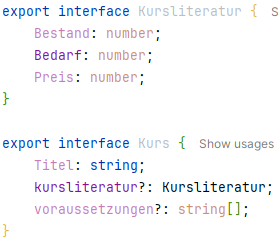
\includegraphics{img/types.png}
	\caption{Auszug aus unseren Typdefinitionen}
	\label{fig:types}
\end{figure}

Damit diese Typen durchgängig in unserem Anwendungscode verwendet werden, ohne dass wir ständig die Daten beim Schreiben oder Lesen \textit{casten} müssten, haben wir sogenannte \textit{Converter} implementiert. Diese ermöglichen es, typisierte Daten aus der Datenbank zu lesen und wieder zurückzuschreiben – und zwar im Einklang mit den definierten TypeScript-Interfaces.

\begin{figure}[H]
	\centering
	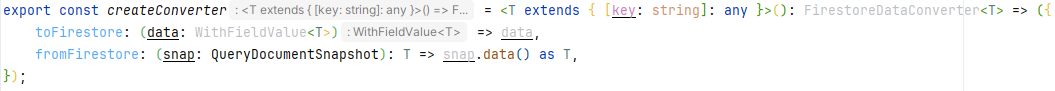
\includegraphics[width=\linewidth]{img/converter.png}
	\caption{Definition unserer \textit{Converter}}
	\label{fig:converter}
\end{figure}

Wie in Abbildung~\ref{fig:converter} zu sehen, implementiert unser \textit{Converter-Objekt} zwei zentrale Methoden: \textit{fromFirestore} konvertiert das rohe Datenobjekt aus Firestore in einen konkreten TypeScript-Typ, während \textit{toFirestore} dafür sorgt, dass nur strukturkonforme Objekte in die Datenbank geschrieben werden \cite{FirebaseConverter.2022}. 

Im Zusammenspiel mit der Methode \textit{.withConverter()} des Firestore-SDK konnten wir so eine durchgängige Typprüfung bei allen Lese- und Schreibvorgängen realisieren. Abbildung~\ref{fig:converter_example} zeigt ein Beispiel für den praktischen Einsatz des \textit{Converters} im Code:

\begin{figure}[H]
	\centering
	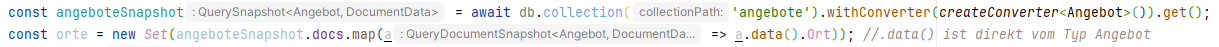
\includegraphics[width=\linewidth]{img/converter_example.png}
	\caption{Beispiel für die Verwendung eines \textit{Converters}}
	\label{fig:converter_example}
\end{figure}

\paragraph{\textbf{Praktische Vorteile.}} Der Einsatz dieser Technik brachte mehrere Vorteile mit sich:

\begin{itemize}
	\item \textbf{Reduktion von Fehlern:} Typfehler, vergessene Felder oder falsche Datentypen wurden bereits zur Entwicklungszeit durch den TypeScript-Compiler erkannt.
	\item \textbf{Bessere Wartbarkeit:} Änderungen an Datenstrukturen waren dank der zentralen Typdefinitionen leicht nachvollziehbar und systemweit konsistent anpassbar.
	\item \textbf{Konsistenz in beiden Richtungen:} Die gleiche Datenstruktur wurde sowohl beim Einlesen als auch beim Schreiben verwendet – ohne doppelte Validierung oder manuelle Typzuweisungen.
\end{itemize}

\paragraph{\textbf{Abgrenzung zum Firestore-Modell.}} Firestore selbst stellt – anders als relationale Datenbanken – kein festes Schema zur Verfügung. Durch die Kombination aus TypeScript und \textit{Convertern} konnten wir dieses Defizit vollständig auf Anwendungsebene kompensieren. Besonders im Rahmen der Migration einer bestehenden SQL-Datenbank erwies sich dieser Ansatz als äußerst hilfreich.

\section{Initiales Laden der Daten nach Firestore}

Nachdem die Datenstruktur definiert und die Nutzung von TypeScript-Typen sowie \textit{Convertern} zur Gewährleistung der Typsicherheit erläutert wurde, bestand der nächste Schritt darin, die Ausgangsdaten in die Firestore-Datenbank zu überführen. Dies war notwendig, um anschließend alle \textit{read}-, \textit{update}- und \textit{delete}-Operationen ausführen zu können.

Die bereitgestellten Daten wurden zunächst in mehreren \textit{.json}-Dateien organisiert. Mithilfe eines eigens entwickelten \textit{Load-Skripts} konnten diese anschließend automatisiert in Firestore importiert werden. Dabei war es entscheidend, dass für jede Datei der passende \textit{Converter} in Kombination mit den zuvor definierten TypeScript-Typen verwendet wurde.

Besonderes Augenmerk lag auf der korrekten Behandlung von \textit{Sub-Collections}, da diese – anders als in relationalen Datenbanken – nicht automatisch mit dem Hauptdokument gespeichert werden, sondern explizit separat geschrieben werden müssen. Abbildung~\ref{fig:load_example} zeigt die Schritte zum initialen Laden der Kurs-Daten nach Firestore auf:

\begin{figure}[H]
	\centering
	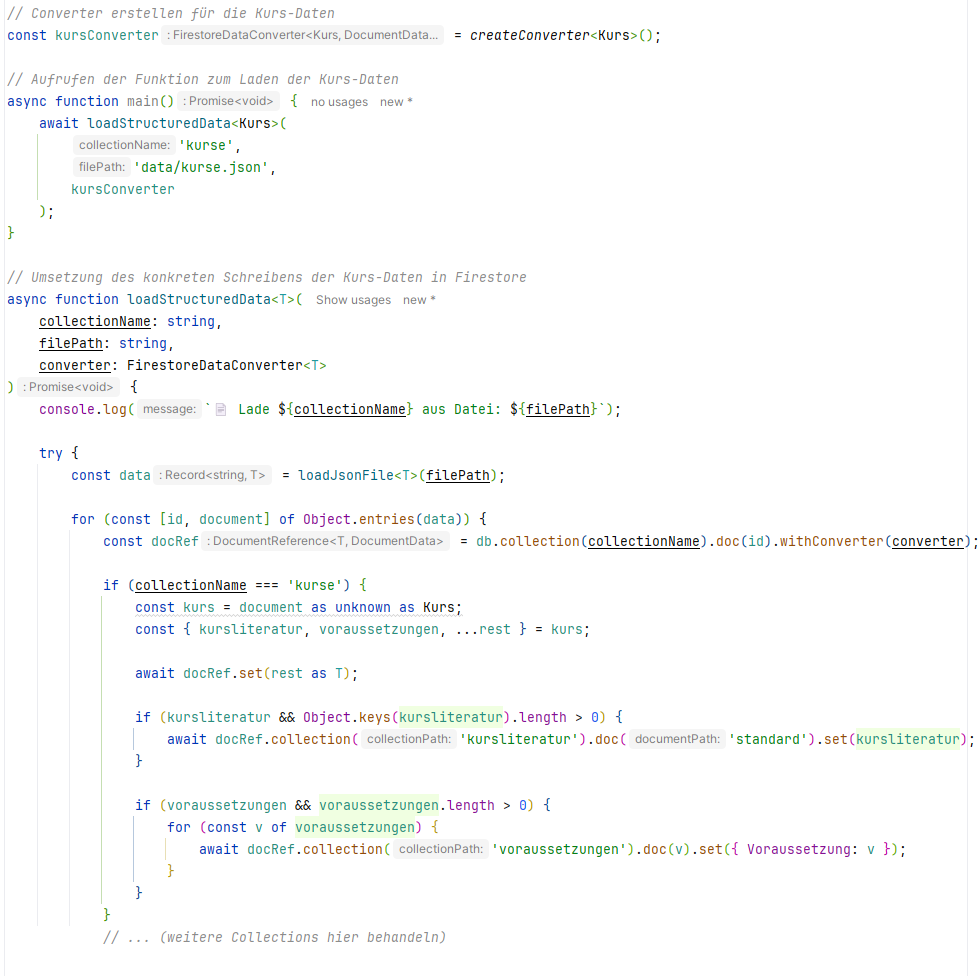
\includegraphics[width=\dimexpr0.9\linewidth]{img/schreiben_beispiel.png}
	\caption{Beispiel für das Laden der Daten in die Firestore Datenbank}
	\label{fig:load_example}
\end{figure}

Abbildung~\ref{fig:load_example} zeigt die Erstellung des \textit{Kurs-Converters}, der anschließend in der \textit{main-Methode} des TypeScript Skripts genutzt wird, um die \textit{kurse.json} mithilfe der \textit{loadStructuredData} Funktion nach Firestore zu schreiben. Hierbei werden in der Funktion die einzelnen Schritte für die \textit{Sub-Collections kursliteratur und voraussetzungen} ebenfalls veranschaulicht, um die gesamten Kurs-Daten ordnungsgemäß initial zu laden.

Obwohl dieser Initialimport technisch gesehen relativ einfach umzusetzen war, musste er sehr sorgfältig durchgeführt werden, um sicherzustellen, dass sämtliche Daten im richtigen Format und an der korrekten Stelle gespeichert werden. Nur so konnten wir garantieren, dass alle nachfolgenden Abfragen erwartungsgemäß funktionieren.

\chapter{Herausforderungen bei den Read-Abfragen}

Bei der Umsetzung der Leseabfragen in Firestore traten mehrere Einschränkungen zutage, die im Vergleich zu klassischen relationalen Datenbanken zusätzliche Komplexität mit sich brachten. Im Folgenden sind drei zentrale Punkte exemplarisch erläutert, die in unserem Projekt den meisten Einfluss hatten:

\begin{enumerate}
	\item \textbf{Keine Unterstützung für \textit{JOINs}:} 
	In SQL können Daten aus mehreren Tabellen mithilfe von \textit{JOIN}-Operationen direkt miteinander verknüpft werden. In Firestore existiert eine solche Funktionalität nicht. Um beispielsweise die Informationen über Teilnehmer zu erhalten, die einen Kurs am eigenen Wohnort gebucht haben (Aufgabe g) müssen mehrere Leseoperationen mit clientseitiger Logik durchgeführt werden, um den gewünschten Output zu erhalten. Nachfolgend veranschaulicht Abbildung~\ref{fig:join_example} die konkrete Umsetzung der Aufgabe \textbf{g)} auf Grund von fehlender \textit{JOIN}-Funktionalität in Firestore:
	
	\begin{figure}[H]
		\centering
		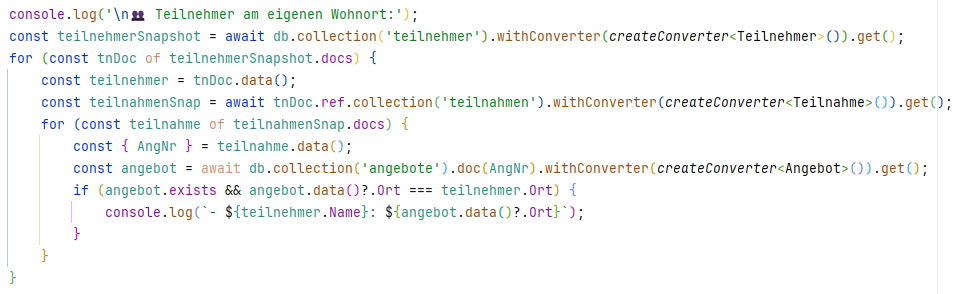
\includegraphics[width=\dimexpr0.9\linewidth]{img/g_join_example.png}
		\caption{Umsetzung von \textit{JOINs} in Firestore anhand Aufgabe g)}
		\label{fig:join_example}
	\end{figure}
	
	Dies führt bei größeren Datenmengen zu einem erheblichen Mehraufwand und einer höheren Anzahl an Leseoperationen – was sich negativ auf die Performance und potenziell auf die Kosten auswirken kann. Wie bereits in Kapitel~\ref{struktur-chapter} (\glqq Aufbau der Datenstruktur\grqq{}) erwähnt, haben wir deshalb zum Teil Redundanzen in unserer Datenstruktur für effizientere Abfragen.\newline
	
	\item \textbf{Eingeschränkte Aggregatfunktionen:}
    Firestore unterstützt inzwischen einfache Aggregationen wie \textit{count()}, allerdings nur für die Gesamtanzahl von Dokumenten, die bestimmte Kriterien erfüllen \cite{FirebaseCount.2025}. Komplexe Aggregationen wie \textit{GROUP BY} oder \textit{HAVING COUNT(*)}, wie sie in SQL üblich sind, sind in Firestore weiterhin nicht möglich. In Aufgabe \textbf{i)} (Kurse mit mindestens zwei Teilnehmern) musste daher in Firestore ein eigenes Zählerobjekt im Anwendungscode erstellt werden, das sämtliche \textit{Teilnahme-Dokumente} durchläuft und die Anzahl pro Kursangebot manuell berechnet. Nachfolgend veranschaulicht Abbildung~\ref{fig:agg_example} die konkrete Umsetzung der Aufgabe \textbf{i)} auf Grund von fehlender eingeschränkter Aggregatfunktionen in Firestore:
    
    \begin{figure}[H]
    	\centering
    	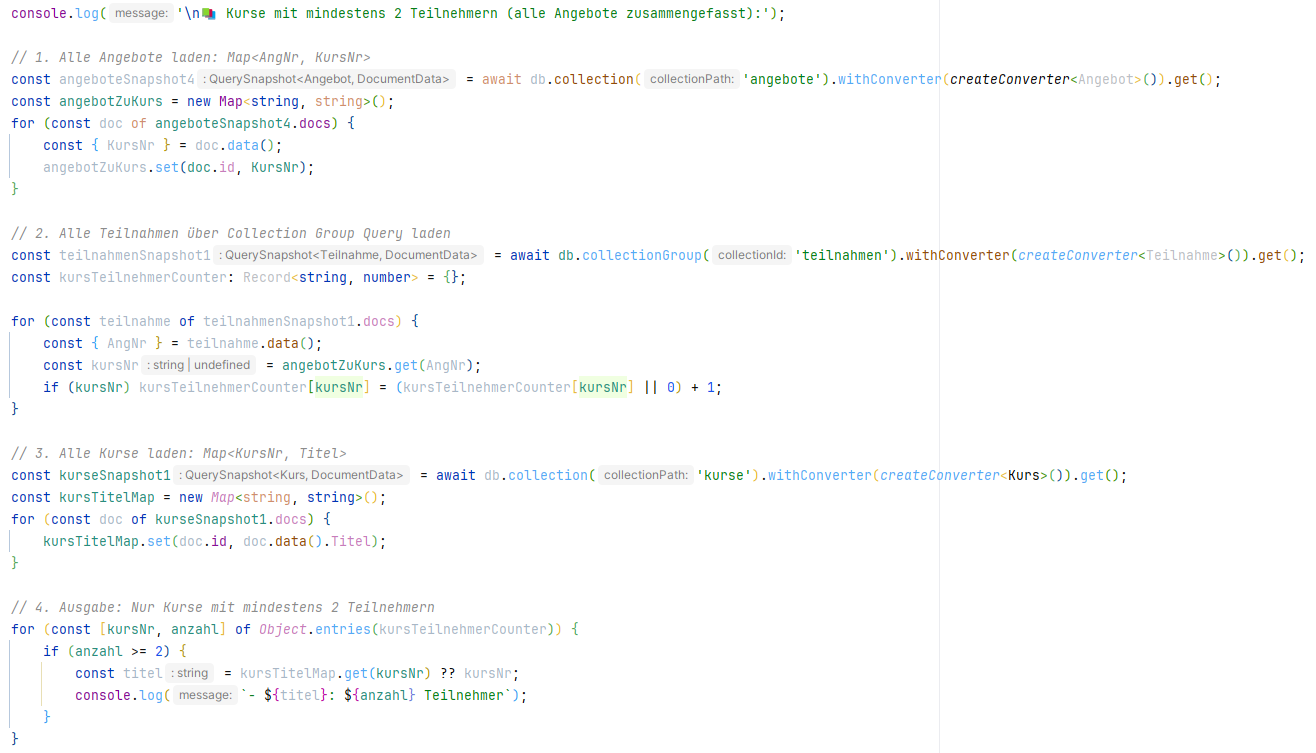
\includegraphics[width=\dimexpr0.9\linewidth]{img/zaehlerobjekt.png}
    	\caption{Umsetzung von \textit{Count} in Firestore anhand Aufgabe i)}
    	\label{fig:agg_example}
    \end{figure}
    
    Das verlagert die Logik vollständig in die Anwendungsebene und erhöht damit den Entwicklungsaufwand. \newline
     
    \item \textbf{Kein direkter Zugriff auf \textit{Sub-Collections} innerhalb \textit{Collections}:}
    In Firestore ist der direkte Zugriff auf \textit{Sub-Collections} nicht ohne Weiteres möglich – etwa, wenn man aus einer übergeordneten \textit{Collection} alle enthaltenen Sub-Dokumente aggregiert betrachten möchte. Auch hierfür sind zusätzliche Leseoperationen und individuelle Nachladeprozesse erforderlich. Das liegt daran, dass Abfragen in Firestore \glqq flach\grqq{} sind und nur Dokumente aus einer bestimmten Sammlung oder Sammlungsgruppe zurückggeben werden können und keine Daten aus untergeordneten Sammlungen \cite{FirebaseComparison.2025}.
    
    Dadurch entstehen, insbesondere bei komplexeren Abfragen wie den Teilaufgaben \textbf{m)} und \textbf{n)}, in Schleifen verschachtelte mehrfache Datenbankzugriffe. Durch Anpassung unserer Datenstruktur und die Speicherung von Informationen redundant, konnten wir hier etwas entgegenwirken und die Anzahl der Iterationen verringern (siehe Kapitel~\ref{struktur-chapter}: \glqq Aufbau der Datenstruktur\grqq{}). 
    
    Will man allerdings für alle gleichnamigen \textit{Sub-Collections} eine Operation ausführen, bei der die Informationen der \textit{Haupt-Collection} keine Rolle spielen, z.B. in unserem Fall die gesamt Teilnahmen eines Angebots betrachten, ist das direkt möglich und ohne mehrfache Nachladeprozesse. Hierzu stellt Firestore den Befehl \textit{collectionGroup} bereit, der alle gleichnamigen \textit{Collections} in der ganzen Datenbank direkt lädt \cite{FirebaseSammlung.2025}.
\end{enumerate}

Diese Einschränkungen zeigen exemplarisch, dass NoSQL-Systeme wie Firestore zwar flexibel in der Datenmodellierung sind, jedoch bei komplexeren Auswertungen oft zusätzliche clientseitige Logik erforderlich machen.

\chapter{Herausforderungen bei den Update- \& Delete-Abfragen}
\label{update-delete-chapter}

Bei den gestellten Update- und Delete-Aufgaben handelte es sich um sehr einfache, die zum Großteil jeweils nur eine \textit{Collection} betrafen und sehr einfach durchgeführt werden konnten. 

Hätte es sich um Update- oder Delete-Abfragen gehandelt, die mehrere \textit{Collections} betroffen hätten bzw. Daten, die von uns mehrfach gespeichert werden, dann wären wir auf neue Herausforderungen gestoßen, um Datenintegrität zu gewährleisten, da es bei Firestore kein \textit{ON DELETE CASCADE} oder \textit{ON UPDATE CASCADE} gibt. Nachfolgend wird ein genau solches Beispiel für den Delete-Fall, der aber auch identisch auf die Update-Operation übertragen werden kann bei der Umsetzung, aufgezeigt, um zu veranschaulichen, wie man solche Probleme mit Firestore umsetzen würde.

\paragraph{\textbf{Beispiel}: Löschen von einem Angebot}
Wird ein Dokument in einer \textit{Haupt-Collection} gelöscht (z. B. das Angebot für einen bestimmten Kurs), so bleiben zugehörige Dokumente in \textit{Sub-Collections} oder redundanten Kopien (etwa in Teilnehmer/Teilnahmen) bestehen – es sei denn, sie werden explizit mitgelöscht. Das kann zu Inkonsistenzen und verwaisten Daten führen, wenn keine zusätzliche Logik zur Datenpflege implementiert wird.

Zur Umsetzung konsistenter Löschvorgänge muss also anhand einer eigenen Lösch-Logik-Implementierung festgelegt werden, dass alle zugehörigen Dokumente, Sub-Dokumente und Kopien ebenfalls gelöscht werden. Um dies zu verdeutlichen, beziehen wir uns direkt auf das Löschen eines Angebots in diesem Projekt. In diesem Fall muss nicht nur das Angebot selbst, sondern zusätzlich alle zugehörigen Teilnahmen und Gebühren sowie der redundant gespeicherte Kursleiter im Angebot entfernt werden.
Ein Vorteil unserer Datenspeicherung liegt in der Speicherung der Teilnahme zusammen mit den Gebühren direkt im Teilnehmer-Dokument. Dadurch müssen wir lediglich die zugehörigen Teilnahmen, vom betroffenen Angebot löschen, um auch die Gebühren zu entfernen.

Da hier grundsätzlich oft ein hoher Aufwand von Schleifen-Operationen (z. B. for-Schleifen) und darin enthaltenen Löschvorgängen zu Grunde liegt, bietet sich das Konzept der \textit{Transaktionen} und \textit{Batch-Operationen} \cite{Firebase.TransaktionenBatch} in Kombination für die Durchführung der Lösch-Operation an. Firestore ermöglicht es, mehrere Löschvorgänge in einer Transaktion zu bündeln, sodass sie entweder alle erfolgreich ausgeführt oder im Fehlerfall zurückgerollt werden. Dies stellt sicher, dass die Datenbank in einem konsistenten Zustand bleibt und keine Teilergebnisse hinterlässt.
Dabei gilt es zu beachten, dass Firestore vorgibt, dass Lese-Operationen immer vor Schreib-Operationen in den Transaktionen stehen müssen und eine maximale Anfragegröße von 10 Mebibyte (MiB) pro Transaktion gilt.
Nachfolgend zeigen Abbildungen~\ref{fig:transaction-1}, \ref{fig:transaction-2} und \ref{fig:transaction-3} die nötigen Schritte auf, um eine Kombination aus einer \textit{Transaktion} und \textit{Batch-Operationen} für die ordnungsgemäße Löschung eines Angebots:

\begin{figure}[H]
	\centering
	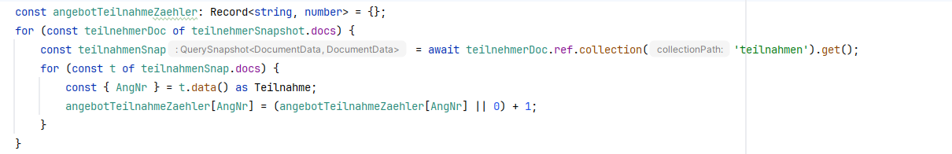
\includegraphics[width=\linewidth]{img/transaction_1.png}
	\caption{Schritt 1: Angebote und Teilnehmer extrahieren}
	\label{fig:transaction-1}
\end{figure}

\begin{figure}[H]
	\centering
	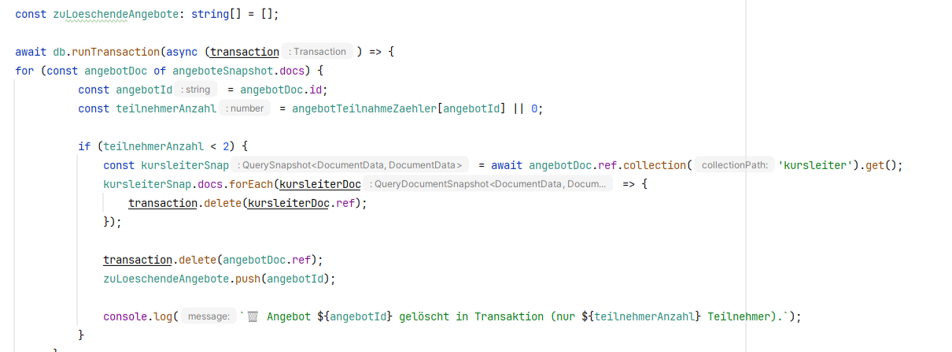
\includegraphics[width=\linewidth]{img/transaction_2.png}
	\caption{Schritt 2: Transaktion starten und Angebot Dokument löschen}
	\label{fig:transaction-2}
\end{figure}

\begin{figure}[H]
	\centering
	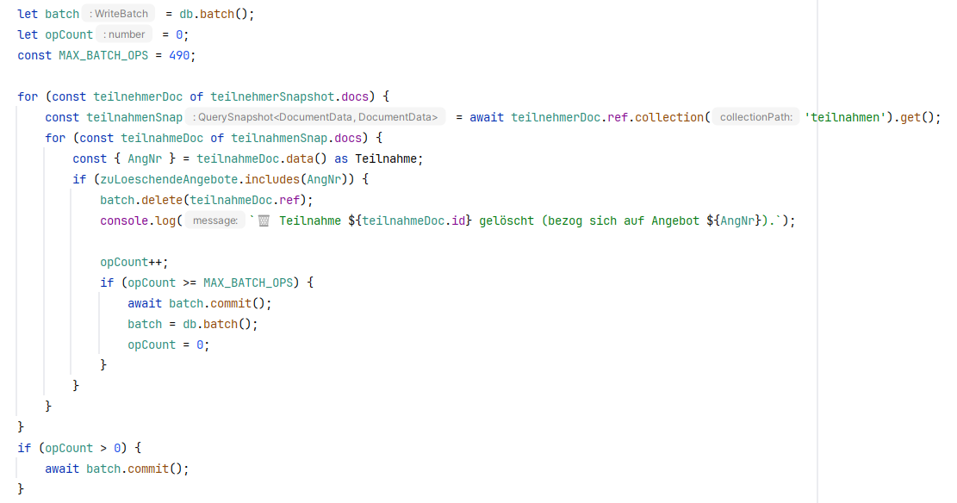
\includegraphics[width=\linewidth]{img/transaction_3.png}
	\caption{Schritt 3: Alle Teilnahmen durchlaufen und zugehörige auf Lösch-Liste der Batch-Queue setzen mit commit für Durchführung am Ende}
	\label{fig:transaction-3}
\end{figure}

Alternativ könnte mit einem serverseitigen Mechanismus \textit{Firebase Cloud Functions} \cite{Firebase.CloudFunctions} gearbeitet werden. Diese \textit{Functions} reagieren automatisch auf Datenänderungen - wie beispielsweise in diesem Projekt einen Löschvorgang eines Angebots. Nachfolgend zeigt Abbildung~\ref{fig:cloud-function} die Umsetzung einer solchen \textit{Cloud Function}:

\begin{figure}[H]
	\centering
	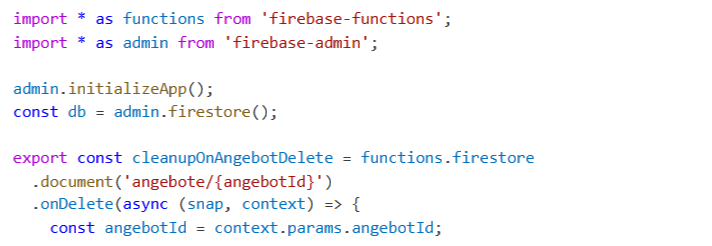
\includegraphics[width=\dimexpr0.8\linewidth]{img/cloud_function.png}
	\caption{Umsetzung einer \textit{Cloud Function} mit Trigger beim Löschen eines Angebots}
	\label{fig:cloud-function}
\end{figure}

Diese Lösung war in unserem Projekt jedoch nicht erlaubt, da ausschließlich lokal mit der Emulator Suite gearbeitet wird und dementsprechend keine Cloud-Integrationen erlaubt sind.

Somit liegt die Verantwortung für konsistentes Löschen bei der Anwendungsschicht. Diese Tatsache ist ein bedeutender Unterschied zu relationalen Systemen, der insbesondere bei komplexeren Datenmodellen berücksichtigt werden muss.

\chapter{Fazit}

Die Migration einer relationalen Kursdatenbank in eine dokumentenbasierte NoSQL-Datenbank wie Google Cloud Firestore stellte sich als ebenso herausfordernd wie lehrreich heraus. Während relationale Datenbanken durch ihr starres Schema und eingebaute Beziehungen wie \textit{JOINs}, \textit{GROUP BY} oder referenzielle Integrität eine hohe Datenkonsistenz und Abfrageflexibilität bieten, verlangt das Arbeiten mit Firestore ein grundsätzlich anderes Denken: Daten müssen häufiger redundant gespeichert, Abfragen logisch vereinfacht und viele Operationen in die Anwendungsschicht verlagert werden.

Durch die Verwendung von \textit{TypeScript} und \textit{Convertern} konnten wir diesem schemalosen Ansatz eine starke Typsicherheit entgegensetzen und so sowohl bei der Datenmodellierung als auch bei der Datenverarbeitung präzise und konsistente Strukturen gewährleisten. Besonders hilfreich war dieser Ansatz im Kontext der ursprünglichen relationalen Struktur, da wir so viele der alten Konzepte typisiert beibehalten konnten.

Die Herausforderungen im Bereich der Lese-, Update- und Delete-Operationen haben deutlich gemacht, dass NoSQL-Systeme zwar hohe Flexibilität bieten, dafür aber auf Kosten automatischer Konsistenzmechanismen und vor allem Performanz. Durch manuelle Skripte und gezielte angepasste sowie redundante Datenmodellierung konnten wir hier aber ebenfalls viel erreichen und den Einschränkungen entgegenwirken.

Abschließend lässt sich sagen, dass dokumentenbasierte Datenbanken wie Firestore ideal für Projekte mit semistrukturierten Daten und klar definierten Zugriffsmustern geeignet sind. Das Projekt hat nicht nur unsere Kenntnisse in Firestore, TypeScript und NoSQL-Datenmodellierung vertieft, sondern auch ein praktisches Verständnis dafür geschaffen, wie sich ein klassisches relationales Datenbankmodell in eine moderne, flexible NoSQL Datenbank überführen lässt.


\appendix

% Selbständigkeitserklärung
%\AuthorDeclaration


%\listoffigures % Abbildungsverzeichnis
%\listoftables % Tabellenverzeichnis

% --------------------------------------------------
% Bibliographie
% --------------------------------------------------
\renewcommand{\bibfont}{\footnotesize}
\printbibliography[title={Literaturverzeichnis}, 
                   heading=bibintoc]


% --------------------------------------------------
% Index
% --------------------------------------------------
{\setkomafont{section}{\Huge} % temporarily set chapter font
\printindex
}

\end{document}
